\chapter*{Introdução\smallskip\subtitulo{Olhar para os Hupd'äh}}
\addcontentsline{toc}{chapter}{Introdução, \textit{por Danilo Paiva Ramos}}

\setlength{\epigraphwidth}{.40\textwidth}
\begin{epigraphs} 
\qitem{Se va enredando, enredando\\
como en el muro la hiedra\\
y va brotando, brotando\\ 
como el musguito en la piedra\\
como el musguito en la piedra,\\
ay si, si, si
}{\textsc{violeta parra}, \textit{Volver a los 17}}
\end{epigraphs}

\section{Viagem ao Tiquié}\label{viagem-ao-tiquiuxe9}

As águas escuras escorrem por entre as árvores. Caminhos líquidos pisam
e repisam o solo da densa mata. Esculpem os contornos das paredes de
madeira e folhas. Os rios negros traçam seus rumos. Curvam"-se centenas
de vezes diante da mata verde. Do céu, os rios grandes rastejam como
cobras por entre as dobras da floresta amazônica. A janela do avião
revela ao estrangeiro um mundo desconhecido e vasto. Nos abismos dessa
vertigem selvagem, impossível não sentir os olhos arregalarem"-se e uma
sensação de insignificância e de fascínio percorrer o corpo. Livros,
fotografias, imagens de documentários, nada parece traduzir esse
universo imenso e pleno de possibilidades de existência e vida.

Num instante, a pequena clareira avistada do alto transforma"-se numa
cidade amazônica, São Gabriel da Cachoeira. O pequeno avião aterrissa
num aeroporto militar, herança dos governos ditatoriais. Ao sair, o
viajante sente o ar úmido em seus pulmões e o calor do sol penetrar a
sua pele. No salão, militares, religiosos, comerciantes, pesquisadores,
lideranças indígenas e funcionários do estado saúdam"-se e observam os
que chegam. O asfalto da estrada conduz os carros por vilas periféricas.
A madeira das casas e os telhados de zinco abrigam aqueles que vieram de
longe. Os moradores viviam em comunidades nos rios Tiquié, Papuri,
Içana, Negro, Uaupés. Trabalham nas pedreiras, nos sítios, nos areais,
no comércio, nas casas de militares, nos bares, na prostituição, no
tráfico ou onde puderem tirar o sustento da família. Mais à frente
surgem o batalhão do exército, as casas de alvenaria, o ginásio, os
prédios públicos, e a imperiosa Igreja matriz salesiana com seu colégio
acoplado.

%\begin{figure}
%\centering
 % 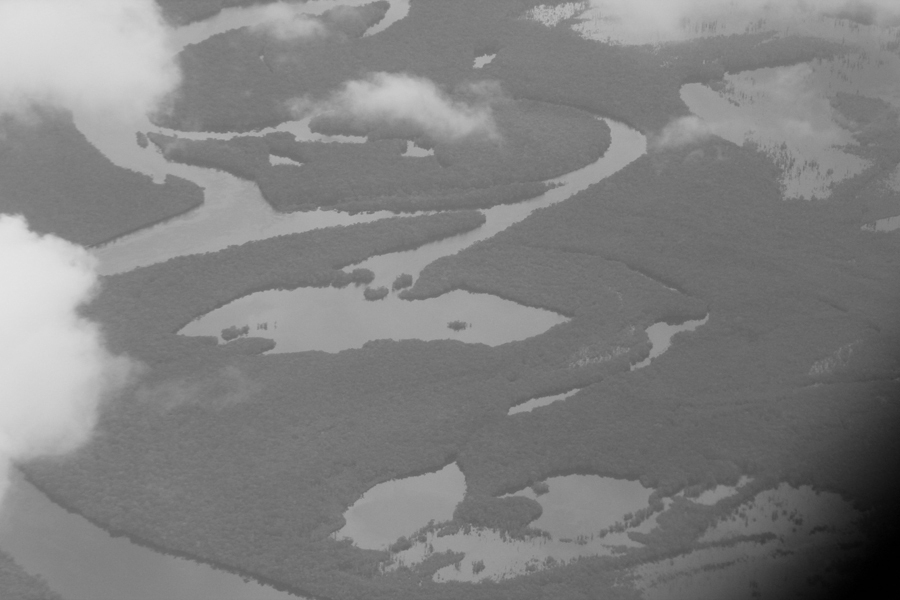
\includegraphics[width=\textwidth]{./img/001}
%\caption{Imagem aérea de afluente do rio Negro (foto: Sylvia C. Novaes, 2012)}
%\end{figure}

A viagem ao Tiquié é adiada a cada dia. A falta de chuvas ou o excesso
de tempestades, o motor quebrado ou a falta de gasolina na cidade, a
doença ou a espera das autorizações de entrada na Terra Indígena fazem
com que o pesquisador fique sempre mais dias no meio urbano do que
imaginava. Em meio a cervejas e caxiris, a pães e beijus, a bifes e
carne de caça, surgem os primeiros laços de amizade. É com indignação
que se começa a ouvir falar da morosidade na demarcação das Terras
Indígenas, da escravidão por dívidas, da violência contra a mulher, da
desatenção à saúde, da falta de estrutura educacional, da corrupção na
prefeitura, do tráfico de drogas. A difícil situação da população local
talvez desperte o desejo de contribuir com o movimento\footnote{A
  Federação das Organizações Indígenas do Alto Rio Negro ({\textsc{foirn}}) é uma
  associação civil fundada em 1987 que se constitui como a principal
  expressão do movimento social e político indígena da região.} e
associações indígenas na busca por melhores condições de vida. No meu
caso, foi também o tempo de acompanhar e assessorar os Hupd'äh em suas
tentativas de obter documentos, benefícios sociais e de participar mais
ativamente do movimento político em busca de melhorias para suas
comunidades.

No porto, a voadeira espera. É chegado o dia da viagem com destino ao
rio Tiquié. Apesar da grande quantidade de roupas, comidas e
equipamentos, resta sempre a sensação de estar se esquecendo de algo.
Acompanhar o dia a dia da pesca, dos trabalhos na roça, das viagens, das
incursões à caça, das festas e das rodas de coca exige a preparação para
inserir"-se em um modo de vida em tudo diferente daquele do morador de
uma grande cidade como São Paulo. Os prédios, as avenidas, as pessoas, a
violência, os barulhos soam aos Hupd'äh como imagens de um meio ao mesmo
tempo estranho, fascinante e perigoso. Nos longos períodos de campo,
minha saudade da família e da esposa comovia sempre meus companheiros.
Queriam integrar"-me a todo custo a seus afazeres, conversar comigo e
nunca me deixar só. Nesse zelo constante, misturavam"-se pena e
solidariedade.

A voadeira vai cortando as águas. O vento forte e o barulho do motor
dificultam as conversas dos tripulantes. Os olhos certamente já estão a
vagar pelo verde das margens. À frente, araras azuis passeiam suavemente
pelo ar. Tucanos pousam nas árvores do lado de lá. Cutucando"-se e
apontando morros, clareiras e aldeias, os companheiros de viagem mostram
lugares, lembram casos e vão ensinando as primeiras lições ao
recém"-chegado. Páginas de livros, imagens de fotografias, cenas de
filmes, palavras de familiares talvez circulem pelos pensamentos do
tripulante. As etnografias lidas falam sobre o povo do barqueiro
Marcelino Massa, um sábio desano que conduz com firmeza o barco.
Denunciam a exploração e violências sofridas pelos parentes barés do
auxiliar de enfermagem Alair Pimenta, que viajou tantas vezes ao meu
lado para atender seus pacientes Hup. Descrevem as guerras combatidas
pelos antepassados de Cecília Piratapuia, ex"-freira, liderança
importante para o fortalecimento da participação feminina na Secretaria
das Mulheres da Federação das Organizações Indígenas do Rio Negro
({\textsc{foirn}}), que sentava"-se mais à proa da embarcação durante a viagem que
fizemos juntos.

Grandes morros de pedra emergem da planície amazônica. O vento forte
parece roubar o som das palavras dos viajantes. O pouco que se escuta
vai transformando as formações rochosas em antigas moradas de heróis
criadores do universo. Algumas clareiras ciliares revelam casas de
alvenaria ou madeira com seus telhados indecisos entre a palha do caranã
e as folhas de zinco da Eternit. Nos arranjos comunitários, uma
igrejinha desbotada sempre faz par com uma escola azul e amarela pintada
há pouco. De povoados desconhecidos, as aldeias passam a ser os sítios
onde vivem diversas pessoas de algum modo ligadas aos tripulantes, entre
primos, amigos, um irmão, conhecidos, um tio"-avô ou uma cunhada.

Com o barulho do motor, as crianças que brincam à beira"-rio correm para
perto de suas casas. No porto, as canoas balançam com o banzeiro de
nossa embarcação a aproximar"-se. Na pequena praia, mulheres de longos
cabelos negros arremessam com força as roupas que lavam contra as
pedras. Um sino toca. A aula vai começar. As crianças saem das casas com
seus uniformes de cor amarela e azul que, na região, chamam"-se
\textit{fardas}, como os uniformes dos militares. O barqueiro desliga o
motor. A voadeira vai vagarosamente empurrando as canoas e ocupando seu
lugar no porto. A fome e a vontade de urinar já tornavam impossível a
continuidade. Num instante, todos arregaçam a barra das calças e pulam
no rio para puxar a voadeira. Monte Alegre era frequentemente o ponto de
nossa primeira parada. O capitão da comunidade vinha cumprimentar os
recém"-chegados e o estranho, o antropólogo, de São Paulo.

Em tempos de seca, quando o rio e os igarapés estão baixos, sempre é
possível trocar sabão, arroz, macarrão e/\,ou sal por peixes moqueados e
beiju. Depois de muitas viagens, os gostos do aracu, da pimenta e do
beiju impregnam na boca a sensação das boas"-vindas. O som das palavras
impenetráveis da língua tukano, falada alegremente pelos viajantes que
reencontram seus conhecidos, passa a ser uma saudação também para
aqueles que aprendem a sentir"-se bem, participando de conversas em
línguas que não compreendem, e a rir de piadas que não podem entender.
Algumas palavras em português permitem seguir a conversa. Por vezes, os
presentes fazem perguntas ao estrangeiro. As novidades da política
local, dos crimes e das festas são comentadas durante o acolhimento e a
partilha da refeição. Pedidos, negociações de trocas e conselhos marcam
a despedida nessas paradas.

A voadeira retoma seu curso. Apenas o barqueiro identifica o caminho a
seguir no espelho d'água. É preciso passar de um lado ao outro para
respeitar o trajeto delimitado pela marinha. Os olhos do barqueiro
perseguem as pedras submersas do rio. Toda atenção é pouca, pois uma
colisão pode emborcar a voadeira e causar uma tragédia. São muitas as
histórias de incidentes envolvendo os barcos mercantes. Numa época de
seca, viajando durante a noite, o barco do comerciante Candinho colidiu
com uma pedra no rio Tiquié. O casco fendeu"-se e a embarcação, com todas
as cargas e bagagens dos tripulantes, afundou. Ninguém morreu, mas foram
muitas as perdas, principalmente das famílias que voltavam de São
Gabriel trazendo roupas, alimentos e instrumentos de trabalho. ``Já vi
muitos barqueiros experientes virarem'', comentou certa vez Marcelino.

Em todas as viagens, em algum momento, nuvens negras começam a
avolumar"-se no céu. A pequena voadeira segue em direção à cortina de
água a ocultar o horizonte. Uma lona azul de {\textsc{pvc}} fornece o abrigo para
que os tripulantes se protejam da força das águas e do vento. Relâmpagos
e trovões iluminam novamente o dia causando temor ao marinheiro de
primeira viagem. O barqueiro veste seu casaco e ajeita seu boné. Segue
firme contra a tempestade. É comum que, depois de horas de precipitação,
o céu volte a se abrir e o sol retome seu brilho. Recolhe"-se a lona,
ajeitam"-se as caixas e os tambores de gasolina da embarcação. Da mata
até o céu, um arco"-íris por vezes contrasta com o cinza das nuvens e com
os diversos tons de verde da mata. Pode ser que uma garça atravesse o
rio bem perto da proa do barco. Branca, desenha no ar um voo rasante.
Pousa sobre uma pedra e acompanha a passagem da voadeira.

Ao longe, avista"-se uma grande igreja. O barqueiro informa que o
distrito de Taracuá se aproxima. O vilarejo é resultado das atividades
dos missionários salesianos. Junto à igreja, uma enfermaria e uma escola
materializam os pilares do projeto civilizatório católico. Velhas
freiras italianas vivem ainda nas casas da missão junto com as freiras
tukano, atualmente em maior número. Certa vez, Cecília contou que nos
anos 1950 o então presidente da república Juscelino Kubitschek pousou de
avião na pista de Taracuá para conhecer de perto as ações missionárias
que, de acordo com o Estado, visavam à integração dos indígenas à
sociedade nacional. Nosso barco parou muitas vezes no porto do vilarejo,
em meio às canoas e a outras voadeiras de alumínio. Precisa"-se descer e
procurar um lugar para dormir, pois o fim da tarde se aproxima e não é
prudente a viagem noturna. Pede"-se ao capitão local a permissão para o
repouso no barracão comunitário. É lá onde dormem os viajantes que
participam dos cursos, reuniões e festas promovidas pelo movimento
indígena. Com um fogareiro preparam"-se os enlatados que se somam ao
peixe moqueado, à pimenta e ao beiju. Redes atadas, todos apagam as
lanternas e deitam"-se com os corpos consumidos pela viagem.

Na penumbra, o sol mal começa a tatear o breu do horizonte e os
viajantes já estão retornando de seus banhos de rio. A refeição matinal
é rápida, pois talvez haja a possibilidade de chegada, no final da
tarde, à comunidade de Taracuá"-Igarapé, nosso destino final. A voadeira
deixa o porto em meio ao vento frio que faz tremer o corpo e ansiar pelo
calor do dia. Depois de uma curva acentuada, o barco despede"-se do rio
Uaupés e penetra as águas do rio Tiquié. As margens estreitam"-se e o
curso d'água revela o tecido rochoso de seu leito. A monotonia do
percurso retilíneo do rio Negro e do Uaupés dá lugar a um itinerário
sinuoso e repleto de paranás. Mais próxima, a vegetação começa a
oferecer"-se menos homogênea em seus tons de verde e de marrom. Flores,
folhas, troncos, arbustos tomam infinitas formas. As trepadeiras,
paxiúbas, paus"-brasil, samambaias, pupunheiras, seringueiras talvez
estejam entre as poucas espécies reconhecidas pelo principiante. No alto
das copas, macacos"-prego, macacos"-barrigudos e provavelmente uma
preguiça se mostram ao viajante.

Nas idas ao Tiquié, talvez uma falha no motor possa reduzir sua
potência. A velocidade passa a ser inferior à metade da empregada em
condições normais, apesar dos esforços do barqueiro em acelerar. O
carburador pode estar sujo. Com sorte, chega"-se à comunidade de Serra do
Mucura antes do pôr do sol para limpar o carburador e descansar. Com a
diminuição da velocidade, acompanha"-se, por alguns instantes, a viagem
das canoas movidas a rabeta. Elas levam os moradores das comunidades do
Tiquié aos vilarejos de Taracuá, Pari"-Cachoeira, outra antiga missão
salesiana, e mesmo a São Gabriel da Cachoeira. Repletas de gente e, em
alguns casos, de caixas com mercadorias, as pequenas embarcações parecem
quase virar a cada ondulação do banzeiro. Com a passagem do barco, todos
que estão na canoa levantam os braços e acenam. Para proteger"-se do sol,
as mães abrigam seus filhos em um guarda"-chuva. As crianças animam"-se
com a passagem da voadeira e sorriem.

Com muito custo, depois de oito horas de viagem, chega"-se à comunidade
de Serra do Mucura. Muitos barqueiros têm fortes laços de amizade com os
moradores dessa aldeia. Alguns dos moradores são considerados ótimos
artesãos e participam do projeto de uma {\textsc{ong}} que criou uma rede de
distribuição e venda de bancos tradicionais nos grandes centros urbanos
do país. O capitão sempre vem ao nosso encontro e nos recebe
calorosamente. Geralmente nos instalamos na casa comunitária onde, sobre
uma mesa, beijus, peixes moqueados e uma quinhampira, caldo de peixe e
pimenta são colocados como oferecimento aos viajantes. Partilhamos a
comida e depois bebemos o chibé, uma refrescante água com farinha. Em
minhas últimas viagens, as eleições municipais e a compra de votos por
parte de alguns candidatos foram temas correntes das conversas e das
piadas. Um dos candidatos, dono de postos de gasolina, distribuíra
combustível de graça para alguns eleitores. Como havia adicionado água à
gasolina, muitas pessoas que voltavam da cidade em suas rabetas ficaram
ilhadas e tiveram que pedir carona para conseguir chegar a suas casas.

À noite, depois do banho, o capitão me fala da vontade que todos têm de
me ouvir tocar violão. Eu começo, então, a dedilhar algumas modas
caipiras. Para minha surpresa, nas minhas primeiras visitas, ouvi os
outros cantarolarem suavemente comigo alguns versos das canções.
``Menino da porteira'' e ``Chico Mineiro'' são sempre as mais pedidas.
Antigamente, as rádios regionais tocavam muito as modas de viola e
familiarizavam os ouvintes com esse estilo musical. Isso permite que meu
repertório seja apreciado com gosto. Por volta das oito e meia da noite, nossos
anfitriões, satisfeitos com a cantoria, despedem"-se e, muito cansados,
retiram"-se para suas casas. Nós atamos nossas redes e rapidamente caímos
no sono.

Logo cedo, a mesa já está repleta novamente de mingau, moqueados e
beijus. Conversamos sobre minha pesquisa e sobre o tempo que eu teria de
permanecer na comunidade de Taracuá"-Igarapé. Como minhas primeiras
incursões à região se deram através do trabalho com saúde pela
Associação Saúde Sem Limites (\textsc{ssl}), em toda conversa falamos muito sobre
os atendimentos das equipes de saúde do \textsc{dsei--rn}. As reclamações sobre as
poucas visitas de atendimento, os remédios vencidos, a demora nos
resgates, a falta de cursos para os Agentes Indígenas de Saúde (\textsc{ais}) e a
falta de médicos dão o tom das falas indignadas. Meu caderno de campo
inicia"-se com notas sobre essas queixas que depois compõem meus
relatórios técnicos em denúncia de tal situação à \textsc{foirn} e ao Controle
Social.\footnote{O Controle Social é uma estrutura composta por conselhos
  nacionais, estaduais e municipais dos quais participam representantes
  comunitários e lideranças de movimentos sociais para fiscalizar a
  condução das políticas públicas em saúde.}

De volta ao barco, nos preparamos para enfrentar o percurso do
Igarapé"-Taracuá, o Ta̗t"-Dëh. Passadas algumas horas de navegação pelo
rio Tiquié, chegamos à comunidade de Cunuri, aldeia tukano onde
atualmente vivem também famílias desano e tuyuka. Um caminho pela mata
leva os cerca de duas horas à aldeia Hup. É para lá que algumas famílias
do Cunuri vão para realizar trocas com os Hupd'äh, demandar auxílio no
trabalho das roças, solicitar que benzedores Hup executem encantamentos,
ou para fazer visitas e participar das festas de caxiri de Ta̗t"-Dëh.
Contam os Tukano que o antigo dono da comunidade foi quem autorizou os
Hupd'äh a constituírem sua aldeia nesse território que consideram seu.
Com a parada no Cunuri, conhecem pessoas tukano que participam da
sociabilidade da aldeia Hup. Ouvem também conselhos sobre a melhor forma
de navegar pelo Igarapé"-Taracuá.

O barco mal entra no Igarapé"-Taracuá e já é possível perceber as
dificuldades que serão enfrentadas no percurso. O caminho d'água
torna"-se estreito e raso. Muitas vezes é preciso que todos desçam do
bote para empurrá"-lo. Em momentos mais difíceis, deve"-se retirar as
caixas de mantimentos e equipamentos para diminuir ainda mais o peso da
embarcação e empurrá"-la com força, para que ela aos poucos vá deslizando
pela areia e encontre área de maior profundidade. Árvores caídas fazem
com que os viajantes desçam com seus terçados para \textit{torar} o tronco
até cindi"-lo ao meio. Toda a atenção é pouca, pois grandes aranhas e
cobras costumam surgir em meio aos troncos e galhos. Vez ou outra, o
barulho do grupo que se aproxima assusta um veado. \textit{Se tivesse uma
espingarda à mão}, lamentam"-se todos.

Passadas longas horas nesse trabalho que exige grande esforço, surge
finalmente o porto de areia da comunidade de Ta̗t"-Dëh. Tendo ouvido já
há horas o barulho do motor de popa, muitas pessoas correm para a beira
para ver e saudar quem está chegando. Depois de algumas viagens, foi com
imensa saudade que passei a acenar aos moradores de Ta̗t"-Dëh, que foram
se tornando grandes amigos. Do estranhamento das primeiras estadas,
comecei também a perceber os sorrisos e cumprimentos afetuosos depois de
meses de distância.

Passei a entender também que meus interlocutores são, antes de mais
nada, viajantes sedentos pelas notícias das terras distantes. O
desbravamento das muitas ``coisas dos brancos'' como carros, cachaças,
casas, comidas, roupas, músicas, filmes vem ocorrendo através das
constantes viagens a São Gabriel. Essas idas ao centro urbano
alternam"-se com as andanças pela mata para a pesca, caça e visita a
parentes, que são também uma fonte inesgotável de causos e lembranças.
Mas suponho que o gosto pelas notícias que eu trazia e o interesse por
São Paulo tenham algo a ver com a própria história de origem de seus
ancestrais, os \textit{hib'ah te͂h d'äh}. Saídos do Rio de Janeiro, do
Pu̗d"-dëh"-moh, o Lago"-de"-leite, os antepassados dos Hupd'äh viajaram
por muito tempo dentro da M'e̖h Hõh Tëg, a Cobra"-Canoa. Depois de
ter chamado os seres humanos à existência, K'e̖g Te͂h fez a Cobra"-Canoa
e mandou que todas as Gentes"-Peixe embarcassem e rumassem para a região
do Uaupés. Alguns não aguentaram a viagem longa e penosa, caíram da
Cobra"-Canoa e vivem hoje nas Dëh"-Mo̖y, Casas"-do"-Rio, que existem
nas profundezas dos rios Negro, Uaupés e Tiquié. Esses continuaram a ser
Gente"-Peixe, não se transformaram em Hupd'äh e, por isso, causam doenças
e vivem tentando roubar nossos \textit{espíritos}.

A Cobra"-Canoa foi abrindo o caminho dos rios pelos quais viajamos hoje
em dia. Foi na cachoeira de Ipanoré, Hib'a̖h Hu͂h, que os ancestrais dos
diversos clãs hup emergiram pelos buracos que há nas rochas. Depois da
longa viagem, foi lá que os primeiros Hup sentaram para conversar
enquanto comiam a coca, fumavam tabaco e bebiam \textit{caarpi}. Talvez o
fascínio com que os Hupd'äh contam sobre a viagem de seus antepassados
na Cobra"-Canoa tenha algo desse encantamento com um mundo completamente
diferente daquele que eu vinha experienciando ao longo de minha vida.
Foi com esse encantamento também que comecei a viajar pelos rios da
região do Alto Rio Negro, a sentar"-me nas rodas de coca, a ouvir sobre
as viagens dos antigos, e a andar pelos caminhos das matas.

%\begin{figure}
%\centering
 % 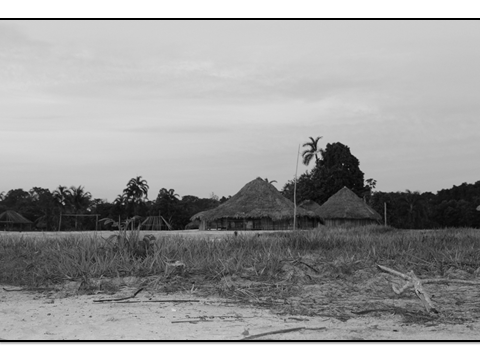
\includegraphics[width=\textwidth]{./img/002}
%\caption{Vista da aldeia de /Ta̗t"-dëh/ (Foto: Sylvia C. Novaes, 2012)}
%\end{figure}

\section{Encontros noturnos e caminhos
vividos}\label{encontros-noturnos-e-caminhos-vividos}

O velho Henrique está morto. A notícia chegou naquela tarde por
\textit{e"-mail}. A fumaça do cigarro deixava minha boca e tateava
lentamente o ar frio. O traumatismo craniano ocasionado por uma queda no
banheiro mal equipado do posto de saúde fez com que ele morresse dias
depois do acidente. Como aprendi, seu espírito viajava naquele momento
para a Paç Pö̗g, a Serra Grande, onde coabitaria com seus
antepassados. Mais tarde, ascendendo, o percurso o levaria à casa do
criador, K'e̖g Te͂h. ``No próximo ano não estarei mais aqui'', ele me
disse em língua hup no momento em que o abracei, despedi"-me, e dei a ele
minha rede. O calor da febre e as tosses causadas por uma forte gripe
não o deixavam descansar. Uns dias antes, ele acordou triste e contou ao
filho um sonho. Tinha sido levado para o fundo da Terra pelos K'öd
d'äh. Disse a eles que não era de lá. Mandaram que seguisse um
beija"-flor/canoa para chegar novamente à Terra. Acordou triste. O sonho
mostrava que seu \textit{ha̗͂wäg}, ``espírito'', estava deixando seu corpo. Eu
não poderia mais acender seus cigarros, ouvir suas histórias nas rodas
de coca nem cantar com ele os \textit{caapivaiás}.

O velho Henrique\footnote{\textit{B'o̖'}, falecido, \textit{Sokw'ä̗t Noh K'öd Tẽ̖h}.} foi
a primeira pessoa Hup que conheci logo que cheguei à cidade de São
Gabriel da Cachoeira, em 2007. Ficamos juntos alojados na casa da
Associação Saúde Sem Limites (\textsc{ssl}), onde ele recebia cuidados médicos e
eu aguardava a viagem com a equipe da \textsc{ong} para realizar um diagnóstico
participativo em comunidades Hup quanto aos impactos da suposta
sedentarização sobre a saúde e a qualidade de vida dessa população.
Almoçávamos e jantávamos juntos e, de alguma forma, nos comunicávamos,
cantávamos e fazíamos companhia um ao outro. Quando comecei meu trabalho
de campo em 2009 na aldeia de Taracuá"-Igarapé, Ta̗t"-Dëh, tomávamos café
pela manhã, comíamos juntos no início da tarde, cantávamos e gravávamos
os cantos do \textit{caapivaiá} e, no início da noite, íamos participar dos
encontros noturnos para comer coca, fumar, ouvir histórias e
benzimentos. Acredito que esse laço que nos unia esteja relacionado com
o modo como foram se estabelecendo os contornos da etnografia sobre as
rodas de coca e os caminhos vividos pelos Hupd'äh.

Ao pôr do sol, quando o som do pilão começa a soar na aldeia, é possível
acompanhar os passos dos senhores Hup que vão caminhando vagarosamente e
se reunindo atrás de uma casa na periferia da comunidade. Alguns
encontram banquinhos. Outros repousam seus corpos sentando no chão de
areia. Aos poucos, é possível ver uma roda surgir em torno do pilão que
vai triturando a coca e as folhas queimadas de imbaúba. Enquanto isso, a
fumaça cinza vai se espalhando pelo ar e cigarros movimentam"-se nas
bocas. As saudações são acompanhadas de risos e piadas, e seguidas por
comentários sobre as andanças pelos caminhos para a pesca, caça ou
colheita de folhas de coca. A mistura de coca e imbaúba é então
derramada numa cuia que começa a circular de mão em mão. Lembro"-me de
que o velho Henrique era sempre o primeiro a receber a coca por ser o
mais velho da comunidade. Cada participante vai derramando a coca na
boca à medida que histórias são contadas e encantamentos ensinados.
Murmurando palavras para cigarros ou cuias, alguns dos presentes começam
também a executar ações xamânicas para curar ou proteger pessoas.

A pesquisa de campo foi realizada principalmente na comunidade Hup de
Taracuá"-Igarapé, Ta̗t"-Dëh, na qual habitam aproximadamente 202
indivíduos e que está situada em território hup às margens do igarapé de
mesmo nome, afluente do rio Tiquié. Há, ao todo, vinte e seis casas onde
moram 38 grupos domésticos. O clã Sokw'ä̗t Noh K'öd Tẽ̖h é majoritário e
reivindica a posse do território, das áreas de caça, pesca e roça. Há
também a presença de muitas famílias que, na geração atual, se
identificam como pertencentes ao clã Dög M'e̖h Tẽ̖h D'äh, grupo afim aos
Sokw'ä̗t Noh K'öd Tẽ̖h D'äh. Essas famílias dizem ter pertencido
anteriormente à etnia Dâw, mas por diversas razões estão se tornando
Hupd'äh, esquecendo sua língua e benzimentos, casando"-se com pessoas Hup
e assumindo a identidade desse clã. Em algumas noites, mais de uma roda
para o consumo de coca pode se formar. A principal delas ocorre
diariamente e conta com a participação de aproximadamente dez pessoas,
tendo como referência o senhor Ponciano.\footnote{Hu̖d, 5 de julho de 1946, Sokw'ä̗t Noh
K'öd Tẽ̖h.} Uma outra, da qual participam em média 6 pessoas, se
forma próximo à casa do pajé Firmino\footnote{B'o̖', 6 de julho de 1947, Sokw'ä̗t Noh
K'öd Tẽ̖h.} Em Ta̗t"-Dëh, além de Firmino, Armando\footnote{Kä',
5 de janeiro de 1948, Sokw'ä̗t Noh K'öd Tẽ̖h.} também é identificado como
\textit{sä̗w}, ``pajé'', e realiza curas xamânicas. Entretanto, todos os
participantes das rodas praticam o xamanismo, sendo vistos
principalmente como \textit{bi'i̖d d'äh}, ``benzedores''. Dessa forma, tanto
pela intensidade com que se realizam as rodas quanto pela existência dos
pajés e benzedores, essa comunidade mostrou"-se como de especial
relevância para a pesquisa.

Foi sentando"-me às rodas de coca que comecei a ser convidado para seguir
meus interlocutores pelos caminhos que atravessam a floresta. Os
chamados \textit{hup ti̖w}, ``caminhos de hup'', iniciam"-se como continuações
dos trajetos para as roças que vão se estreitando aos poucos até
formarem trilhas fechadas que se diferenciam sutilmente da densa mata.
Seguindo por esses percursos, as pessoas se dirigem diariamente aos
igarapés para a pesca, deslocam"-se para outras aldeias, seguem os
rastros de animais ou realizam viagens para os morros situados nas
cabeceiras. Em meio a seus movimentos, os andarilhos passam pelas
Moy"-Höd, Moradas Antigas, onde seus antepassados habitaram antes
de viver na grande aldeia de Ta̗t"-Dëh. Chegam a lugares impregnados
pela ação de demiurgos cujos feitos são narrados até hoje nas \textit{pɨnɨ̖g},
``mitos'' ou ``histórias''. Descobrem, assim, sentidos imanentes ao mundo que
vão se revelando à medida que os viajantes se situam nessas outras
paisagens e aceitam interagir com animais, plantas, ancestrais e demais
seres com quem coabitam.

Sentados nos encontros noturnos, os senhores Hup revelam"-se viajantes a
narrar seus percursos pelo mundo através dos ``caminhos'', \textit{hup ti̖w}, e
dos deslocamentos xamânicos. O trabalho de campo realizado entre 2009 e
2012 permitiu perceber que as rodas de coca constituem"-se como uma forma
constante de interação central para os fazeres mítico e xamânico, a
partir dos quais os senhores estabelecem relações fundamentais com o
universo hup. Seus movimentos fazem"-nos passar por lugares onde eventos
míticos ocorreram, visitar paisagens habitadas por seres diversos e
praticar ações rituais no alto de morros como a Serra Grande.

Compartilhar as cuias de coca com o senhor Henrique, ouvir seu sonho de
deslocamento para a morada subterrânea dos K'ö̗d däh, testemunhar sua
morte pelo descaso em São Gabriel, e saber de seu percurso póstumo à
Serra Grande motivaram"-me a ocupar um lugar nas rodas e a aceitar seguir
meus mentores em viagens por seus caminhos vividos. Ao longo da
pesquisa, entendi que os encontros noturnos podem ser vistos como um
\textit{modo de ação} que permite aos participantes constituírem
\textit{percursos de observação} a partir de seus próprios movimentos em
meio às palavras sopradas dos encantamentos e aos passos trilhados pelos
caminhos que atravessam a floresta. As rodas de coca, tão importantes
para o senhor Henrique, passaram a ser vistas por mim como
\textit{performances} onde, em meio à sequência dos encontros e viagens,
ocorrem múltiplas \textit{condensações rituais}, tornando determinados
gestos, posturas, palavras e substâncias fundamentais para a interação
com todos aqueles com quem os Hupd'äh partilham paisagens e saberes.
Espero, com esse trabalho, descrever um pouco esses aspectos da
existência dos Hupd'äh que, com a amizade de Henrique, começaram a fazer
parte de minha própria história.

\section{Olhar para os Hupd'äh}\label{olhares-para-os-hupduxe4h}

Os Hupd'äh habitam a região do Alto Rio Negro (\textsc{am}), na fronteira entre o
Brasil e a Colômbia. Suas comunidades situam"-se às margens de igarapés
da área interfluvial dos rios Tiquié e Papuri, afluentes da margem
esquerda do rio Uaupés. Os dados demográficos mais atuais, de acordo com
a pesquisa de Epps (2005) e Athias (2006) estimam a população num total
de 1.500 indivíduos distribuídos em aproximadamente 35 aldeias. A alta
mobilidade e circulação pelo território são aspectos fundamentais do
modo de vida hup, que estão relacionados ao vasto conhecimento que
possuem sobre os caminhos, os igarapés, os animais e a vegetação local.
Associada à mobilidade, a caça"-coleta constitui"-se como foco de
interesse das pesquisas antropológicas sobre esse povo, estabelecendo o
contraste entre os Hupd'äh com as populações ribeirinhas de
pescadores"-agricultores. Ao mesmo tempo, a constância da caça"-coleta tem
diminuído nas últimas décadas, fazendo com que a pesca em igarapés e as
roças de mandioca venham se tornando cada vez mais fundamentais para a
produção alimentar, principalmente nas comunidades mais populosas.
Atualmente, há algumas aldeias que agregam de cem a 200 indivíduos,
enquanto outras continuam concentrando de 15 a 50 pessoas, como parece
ser o padrão descrito pelos pesquisadores. Conforme mostra Athias, em
sua pesquisa de 1995, o aumento populacional e a maior duração da
permanência da morada num local próximo aos grandes rios têm a ver com a
agência missionária salesiana, que procurou agregar em grandes aldeias,
designadas pelo pesquisador como povoados"-missão, o maior número de
pessoas para evangelização.

% \begin{figure}
% \centering
% 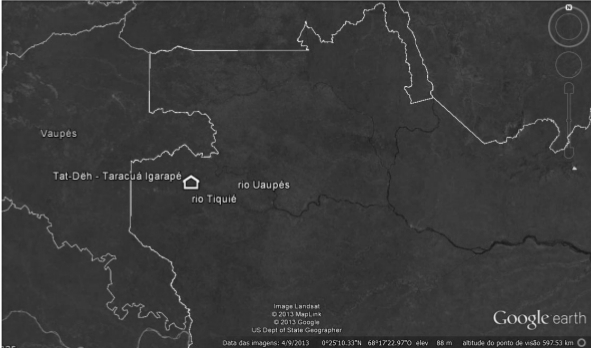
\includegraphics[width=\textwidth]{./img/003}
% \caption{Localização da comunidade Hupd'äh de \textit{Ta̗t"-Dëh},
% Taracuá"-Igarapé}
% \end{figure}

A estrutura social hup tem nos clãs agnáticos seus segmentos básicos de
constituição e de diferenciação. Criados pelo herói cultural K'e̖g Te͂h,
os ``ancestrais'', \textit{hib'a̗h"-tẽ̖h"-d'äh}, deram origem aos hoje
aproximadamente 25 clãs exogâmicos e de descendência patrilinear. Cada
clã possui um conjunto específico de nomes, mitos e cantos por meio dos
quais são narrados os eventos de criação e se constitui um senso de
pertencimento e identidade. O casamento preferencial dá"-se entre os
primos cruzados bilaterais numa mesma geração e procura respeitar certa
hierarquia entre os clãs. Em contraste com outros povos da região, o
sistema de matrimônio dá"-se segundo a endogamia linguística e a exogamia
clânica. O casamento dá origem a grupos de fogo, unidades mínimas de
produção e consumo. A coabitação em um mesmo território ou espaço de
grupos de fogo gera os grupos locais, que são nomeados e diferenciados
entre si. Os deslocamentos de grupos de fogo ou indivíduos para visitas
a parentes de outros grupos locais ocorrem periodicamente e podem durar
meses.

Esses traços aproximam os Hupd'äh de povos como os Yuhupdëh, Nadëb, Dâw,
Kákwa e Nukák, permitindo que fossem designados pela literatura
etnológica da região como povos maku. Entendendo haver um sistema
relativamente homogêneo baseado na exogamia linguística, nas relações
hierárquicas rituais e territoriais entre povos falantes de línguas
tukano e arawak, os pesquisadores descrevem a especificidade da
articulação dos povos maku a esse \textit{sistema vaupesiano}. O próprio
termo \textit{maku}, adotado pela literatura, revela a particularidade dessa
interação, já que a palavra \textit{maku} origina"-se do arawak e significa
``aquele que não tem fala'' ou ``aquele que não tem a nossa fala'',\footnote{\textit{Ma} é um prefixo privativo, e \textit{aku}, ``fala''.} sendo associado a \textit{selvagem}, a
índios"-da"-floresta em oposição a índios"-do"-rio, como os povos tukano e
arawak. A realização de trabalhos nas roças de famílias tukano, que faz
com que famílias maku se mudem para um local próximo às aldeias tukano
em determinados períodos, as trocas de carne de caça e frutos por
mandioca, peixes e mercadorias, e o respeito e silêncio diante dos
tukano são aspectos que fizeram com que os pesquisadores descrevessem as
relações entre esses povos como simbióticas, de patrão--cliente,
hierárquicas--assimétricas.

Segundo a linguista Patience Epps (2005), os traços semelhantes entre as
línguas hup, nadëb (kuyawi), dâw e yuhup constituem"-nas como línguas
irmãs, formando assim uma família linguística. Ela propõe que essa seria
a família nadahup ou, como vem sendo designada por outros estudos, a
família maku. Há também pesquisadores que incluem as línguas kákwa, as bara"-maku, 
e nukák como pertencentes a essa família. O trabalho de
Epps, \textit{A Grammar of Hup}, de 2005, coloca"-se como o primeiro estudo
mais aprofundado da língua hup. Até hoje, a língua hup é a primeira a
ser falada pelas crianças Hup. Dado seu relativo isolamento, poucos
falantes de hup são fluentes em português. Apesar disso, virtualmente
todos são falantes da língua tukano, uma língua tukano oriental falada
pelas etnias próximas que serve como uma língua franca regional. A
partir de 2001, ações da secretaria da educação local e de \textsc{ong}s
implantaram um sistema de formação de professores hup, dâw e yuhup, com
o objetivo de consolidar as escolas desses povos. Começa, a partir de
então, um processo de descrição da língua hup, fixação da grafia,
compreensão dos princípios gramaticais, e alfabetização inicial dos
professores. Foram elaborados um dicionário hupd'äh"-português e
cartilhas na língua hup. Esses materiais vêm permitindo aos professores
desenvolver junto aos alunos a escrita e o aprendizado de sua língua.

% \begin{figure}
% \centering
% 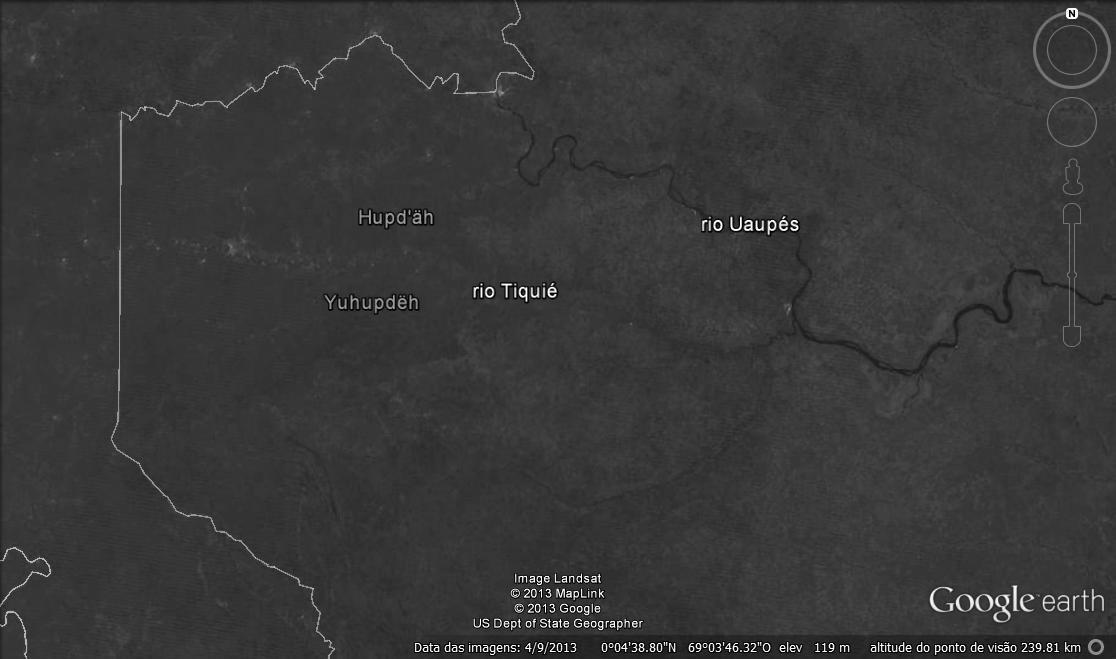
\includegraphics[width=\textwidth]{./img/004}
% \caption{Regiões habitadas por populações das etnias hupd'äh
% e yuhupdëh no médio Tiquié.}
% \end{figure}

O contato teve inicio com as frentes de colonização desde o século
\textsc{xviii}, mas foi apenas nas décadas de 1960 e 1970 do século \textsc{xx} que os
missionários salesianos iniciaram atividades mais intensas visando à
evangelização e à escolarização dos Hupd'äh. Trabalhando já há décadas
com os Tukano, os padres salesianos pretendiam intervir nas relações
vistas como assimétricas entre esses povos. A constituição de aldeias
hup em território tukano e o aumento populacional das comunidades podem
ser vistos como processos influenciados pela ação missionária.
Paralelamente, observa"-se a dificuldade crescente na obtenção de
alimentos, o aumento na taxa de mortalidade e de doenças, e o constante
recrutamento e exploração de mão de obra para a extração de borracha e cipó. 
Nos últimos anos, as atividades das equipes de saúde,
de indigenistas, e de missionários pentecostais vêm somando"-se à ação
dos salesianos que ainda mantêm suas ações em uma aldeia Hup e na região
do Alto Rio Negro como um todo.

\begin{center}
\adforn{68}
\end{center}

Certa vez, enquanto eu lia a tese de Howard Reid em meu computador,
Ricardo se lembrou das histórias do antropólogo que usava tanga, falava
hup, caçava e pescava.

\begin{quote}
Mostrei a Ricardo o livro de Howard Reid. Ele disse que os velhos
falaram pra ele desse que chamavam Haw. Ele usava tanga. Ficava lá no
meio deles. Falava a língua hup. Ia caçar no mato, pescava, fazia tudo
como os Hupd'äh. Ele e o Peter (Peter Silverwood"-Cope). Ele falava pros
velhos que veio de avião. Eles gostavam desse Haw. Mas ele foi embora
e não voltou mais. O avô de Ricardo conheceu"-o. Ele foi embora uns anos
antes de Ricardo nascer.\footnote{(Caderno de campo, datado de 25 de novembro de 2009.}
\end{quote}

Durante minhas estadas em campo, sempre ouço também histórias dos
pesquisadores que me precederam. De formas diferentes, a imagem desses
\textit{brancos} que \textit{viviam com e como os índios} sobrepõe"-se à minha.
Distante das comunidades, encontro"-me com o Haw quase sempre. Seus
trabalhos guiam"-me por muitos percursos florestais que permeiam minhas
experiências partilhadas com os Hupd'äh. Como tenho ouvido em muitas
conversas, a relação com os senhores Hup parece ter sido marcante também
para Reid.

Há poucos trabalhos antropológicos sobre os grupos Maku. Dentre os
existentes, destacam"-se os de Peter Silverwood"-Cope (1972/\,1990) sobre os
Bara"-Maku (Kakwá), de Howard Reid (1979) sobre os Hup'däh, de Renato
Athias (1995) sobre os Hup'däh e Tukano, de Jorge Pozzobon (1983, 1991)
sobre diversos povos maku e, mais recentemente, o trabalho de Pedro
Lolli (2010) sobre os Yuhupdëh. Desses, apenas o trabalho de Reid
apresenta uma monografia extensa sobre os Hupd'äh. Athias enfatiza a
relação interétnica entre os Hupd'äh e os Tukano. Pozzobon (1991), por
sua vez, enfoca os sistemas de parentesco e as regras de casamento dos
Yuhupdëh, Hup'däh, Dâw, Kákwa e Nadëb. Tomando como referência a leitura
crítica da literatura sobre os povos maku feita por Bruno Marques
(2009), passo agora a uma breve discussão a respeito dos trabalhos dos
pesquisadores que se dedicaram ao estudo dos povos Maku.

O primeiro estudo etnográfico detalhado sobre um grupo Maku, os
Bara"-Maku (Kákwa), foi realizado por Peter Silverwood"-Cope em 1972. O
autor salienta que um dos objetivos de sua pesquisa foi o de contribuir
para aumentar o conhecimento sobre os povos Maku, já que era reduzido o
número de pesquisas e eram poucos os dados existentes até então. Antes
de seu estudo, autores como Giacone (1969), Koch"-Grünberg (1906/\,2010),
Biocca (1965) e Münzel (1969) apresentaram apenas listas de palavras,
descrições gerais da cultura material, comportamento e rituais,
transcrições de mitos e resenhas bibliográficas.

Em outubro de 1968, Peter Silverwood"-Cope viajava com Stephen e
Christine Hugh"-Jones para o rio Pira Paraná em busca de grupos Maku na
região. O fato de não ter encontrado tais grupos nessa área fez com que
o antropólogo consolidasse sua pesquisa com um único grupo regional
Bara"-Maku (kákwa), da região do rio Macu"-Paraná. Sua pesquisa apresenta
uma descrição detalhada do modo de vida dos Bara"-Maku e, genericamente,
dos Maku, abrangendo as atividades de caça, pesca, coleta e colheita, os
conhecimentos sobre o ecossistema, técnicas produtivas, sistema de clãs,
regras de casamento e categorias de parentesco. Para descrever a
adaptação ecológica dos Bara"-Maku e mostrar a importância da caça para
esse povo, Silverwood"-Cope observa ser fundamental entender a relação
que os grupos têm em diferentes momentos com a aldeia, o acampamento de
caça e a permanência junto aos Tukano para a realização de trabalhos.

Os padrões de caça são descritos através das técnicas utilizadas, de
dados quantitativos sobre produção e consumo, de formas de classificação
e concepções cosmológicas sobre a atividade. Na monografia, é também
estabelecido o contraste entre a adaptação ecológica tukano e maku, e
são descritas as relações de trocas sociais e econômicas entre ambos. A
complexidade revelada por seu trabalho aponta a necessidade da revisão
da categorização desses povos como sendo caçadores e coletores nômades
muito primitivos que, segundo a literatura científica, vinham sendo
assimilados e escravizados por povos agricultores invasores.

Numa perspectiva semelhante, o trabalho de Reid (1979) busca entender a
cultura e o seminomadismo hup através da mobilidade e da fluidez desse
povo em diferentes espaços da floresta; do seu sistema de classificação
e de relações sociais que marcam as distintas fases da vida, e da sua
cosmologia. As mudanças suscitadas pelas atividades dos missionários
salesianos, pelos comerciantes de produtos extrativistas e pela Fundação
Nacional do Índio (\textsc{funai}) são tematizadas na parte final de seu estudo,
realizado num momento de intensificação do contato.

As atividades econômicas e a organização social são apresentadas sempre
em conexão com os conceitos de mobilidade e fluidez. Além do estudo
sobre economia e organização social, Reid realiza também uma
interessante descrição acerca das fases da vida dos Hup'däh, buscando
sempre relacioná"-las aos espaços sociais e às atividades desempenhadas
por cada um em determinados períodos da vida. Para o autor, as mudanças
nos papéis sociais e nas fases da vida contribuem para aumentar, no caso
dos mais jovens, e diminuir, no caso dos mais velhos, a mobilidade entre
os grupos sociais Hup. Seu trabalho ressalta também a convergência entre
a classificação dos mitos e do cosmos e o sistema de classificação hup
mais geral.

Para Jorge Pozzobon (1983), a principal contribuição das análises de
Reid e Silverwood"-Cope, quanto aos sistemas de parentesco e de
organização social, foi a de revelar que ``o traço mais marcante da
cultura dos povos maku é a grande fluidez com que eles seguem as
próprias regras de aliança e filiação, sua terminologia de parentesco e
suas regras residenciais''. A partir disso, o objetivo de seu trabalho é
enfocar como esse caráter de fluidez dos Maku está ligado a fatores
demográficos.

O autor percebe haver uma tendência geral para que os Maku procurem seus
cônjuges em círculos endogâmicos cada vez mais restritos, estando esse
princípio relacionado à proporção entre os sexos em determinadas
unidades demográficas. Para Pozzobon, a mobilidade desses grupos liga"-se
mais a fatores sociais e políticos do que a fatores econômicos --- caça e
coleta. Os grupos locais funcionam como isolados matrimoniais,
caracterizados pela endogamia e \textit{um sentimento restrito de
identidade}. Assim, o pesquisador parte da diferença entre a suposta
exogamia prescrita pelas regras de matrimônio e a prática cada vez mais
endogâmica evidenciada por seu recenseamento, e analisa o comportamento
fluido desses povos.\footnote{Desse modo, para perceber as dimensões
  relevantes dos sistemas de parentesco e melhor compreender as rodas de
  coca, foi preciso estar atento à diferença entre as regras de
  casamento e à forma como o parentesco se realiza na prática, tendo em
  vista o novo contexto demográfico atual.}

O estudo de Renato Athias, de 1995, analisa as relações interétnicas
entre os Hupd'äh e os Tukano, e as formas de adaptação de cada etnia ao
ecossistema. Contribui para uma melhor compreensão da organização social
e das relações entre esses povos. Segundo ele, a diferença marcante do
sistema de parentesco e das atividades produtivas faz com que as
relações interétnicas se caracterizem pela assimetria e formem um
sistema hierarquizado. Para o pesquisador, o fato de partir da
perspectiva hup para entender essas relações de subordinação e submissão
com os Tukano faz com que seu trabalho se diferencie das pesquisas
anteriores, que partiam sempre do ponto de vista tukano. Recentemente, o
trabalho de Lirian Monteiro (2011) abordou o tema da relação entre os
Hupd'äh e os Tukano a partir da história da comunidade tukano de
Barreira Alta que, após a migração das famílias tukano para São Gabriel,
passou a ser habitada quase que exclusivamente por famílias Hupd'äh.

Como pode se perceber nas pesquisas já realizadas, as narrativas e ritos
são apenas elementos descritos para a composição de um quadro geral
desses povos, surgindo, geralmente, em capítulos destinados à cosmologia
ou em meio à descrição da organização social desses povos. Assim,
tomando como referência os encontros noturnos enquanto forma de
interação social específica, articulada aos movimentos das viagens, o
trabalho que desenvolvi procura delinear o modo como narrativas e
andanças geram importantes condensações rituais que entrelaçam rodas,
caminhos e paisagens como campos de percepção e ação vividos mutuamente
pelas pessoas Hup.

\section{Movimento de emaranhar}\label{movimentos-de-emaranhar}

Sonhar com uma antropologia livre da desumanização dos sujeitos,
transformados pelos estudos em \textit{portadores impessoais de cultura},
determinados pelas forças, variáveis e pressões sociais foi o que levou
Victor Turner a buscar os estudos da \textit{performance}. Entendendo que
apenas por meio dessa liberdade seja possível escrever sobre os
encontros noturnos revelando os modos de percepção e as sensibilidades
que são por eles mobilizados, descrevo as rodas de coca como sendo uma
\textit{performance} e tento delinear as sequências reflexivas de ações
verbais e não verbais que, noite após noite, geram uma forma constante
de interações.

Ao acompanhar o narrar, o benzer e o andar como sequências articuladas
de modos de ação dos encontros noturnos, abriu"-se a possibilidade de
seguir a organização da ação performática nela mesma através não da
exegese total de um ritual, mas das múltiplas condensações rituais que
associam esses modos de relação. Nesse sentido, a abordagem de Humphrey
e Laidlaw (2004) tornou"-se fértil por permitir ver o ritual como uma
qualidade da ação, e não como uma classe de eventos ou instituições. O
contraste entre ações ritualizadas e ações não ritualizadas ressalta a
importância da atenção do agente para sua própria ação. Essa perspectiva
ajuda a perceber situações surgidas no curso das viagens ou das rodas de
coca como transformações sutis de ações correntes promovidas pelos
caminhantes ou participantes dos encontros. Essas transformações revelam
histórias e características específicas da ação performada que alteram
sentidos, formas de interação e de intenção dos agentes.

Ao longo da pesquisa, percebi que os modos de ação articulados pelas
rodas ocorrem por meio da mobilidade específica das viagens. Essas
viagens são tanto as caminhadas para banhos e ingestão de água das
serras, estas tidas como moradas de ancestrais, quanto os deslocamentos
da pessoa ao benzer ou sonhar, para as casas do céu, do rio, da terra,
onde habitam ancestrais e seres como o Trovão, as Gentes"-Onça, as
Gentes"-Cobra, dentre outros. Pensando com Gow, procuro mostrar como o
interesse dos participantes das rodas por contar um mito ou por executar
um benzimento parte de eventos vividos pelas pessoas ao se deslocarem ao
longo de diversas paisagens pelo mundo. Nesse sentido, foco minha
atenção no mundo vivido, na concretude das experiências vividas pelos
\textit{comedores de coca} como viajantes, agentes"-no"-ambiente que percebem,
atuam, pensam, aprendem e conhecem pelo seu envolvimento mútuo nas rodas
e nos deslocamentos do caminhar e do benzer.

Em seus trabalhos, Lévi"-Strauss mostra como inversões, novas relações,
oposições, ambiguidades e contradições se abrem como feixes de relações
que auxiliam a interpretar questões sugeridas pelos mitos, ritos ou
sistemas de classificação através de mediações progressivas, vistas por
ele como grupos de transformação. Sobre os grupos de transformação de
mitos, o antropólogo diz que ``o sentido de um termo só pode ser
definido substituindo"-o em todos os contextos em que seja encontrado.
{[}\ldots{}{]} o mito é reorganizado de tal maneira que ele próprio se
constitui como contexto'' (Lévi"-Strauss, 2003, p.~247). Partindo de
categorias empíricas definidas por meio da observação etnográfica de
culturas específicas, a análise através dos grupos de transformação
possibilita isolar noções abstratas e encadeá"-las em proposições. Esses
procedimentos seriam fundamentais para explicitar uma lógica das
qualidades sensíveis, em que a inteligibilidade é condição para a
apreensão sensível do mundo. A noção de transformação \textit{levistraussiana}
ajuda a ver inversões, relações, oposições, ambiguidades e contradições
que se dão no curso das ações dos participantes nas rodas e nos caminhos
pela floresta que os fazem gerar transformações. Entretanto, de modo
diferente, essas transformações geradas pelos viajantes Hup não se dão
como \textit{noções abstratas encadeadas}, mas como deslocamentos nas
posições ocupadas em campos mútuos de percepção e ação.

Ao benzer ou caminhar, os \textit{comedores de coca} substituem"-se, por ação
e movimentos, em diferentes ambientes e realizam mediações progressivas
para transformar pessoas ou atitudes dos seres dessas outras regiões. A
noção de plano"-casa proposta por Lolli torna"-se especialmente
interessante para entender esses deslocamentos xamânicos. Há
perspectivas distintas inerentes a cada plano"-cósmico, ou casa, o que
implica numa descontinuidade entre os pontos de vista. Deslocando"-se
entre planos"-casa, a ação dos xamãs gera um contínuo entre planos e
perspectivas à medida que assumem diferentes pontos de vista para
interagir com os habitantes dessas moradas. As viagens xamânicas
permitem também proteger ou curar os Hupd'äh dos malefícios causados
pela circulação de pessoas e de afecções de pessoas pelos diversos
planos"-casa.

Contando sobre os ancestrais, viajando rumo às serras ou aos
planos"-casa, os senhores Hup atuam na passagem entre contextos, na
transição entre estados, na transformação de pessoas e de perspectivas.
Nesse sentido, a abordagem processual de Turner ajuda a perceber como
esses deslocamentos ao longo do mundo resultam em transições e
metamorfoses entre tempos e espaços (\textit{betwixt and beetween}). A
dinâmica constante das ações dos encontros noturnos, ao combinar as
ações mítica e ritual, pode ser vista como um processo por meio do qual
os benzedores constituem"-se como seres transicionais, pessoas liminares.
O aspecto reflexivo das rodas de coca torna"-se mais evidente, já que,
agindo, os participantes, imersos numa pluralidade que os divide entre
Nós e Eles, Ego e Alter, observam e revelam"-se a si
mesmos.

Tomando o trabalho de Gow como referência, entendo ser possível assim
explorar as relações entre os atos de contar, de benzer e de caminhar
como variações, não só de narrativas mas de modos de ação articulados
por \textit{processos de transformação} que se dão pela mobilidade dos
participantes, seja nas viagens aos \textit{lugares sagrados}, seja nos
deslocamentos da pessoa durante os benzimentos por meio de palavras que
agem. Simultaneamente, dado o caráter reflexivo das \textit{performances},
esse processo de transformações leva a uma maior consciência da
habilidade para narrar e benzer, e das dificuldades nos fazeres mítico e
xamânico. Associados pelo contexto relacional particular das rodas,
esses atos também sofrem mudanças com o envelhecimento e com a
participação da pessoa nos encontros noturnos e dos rumos por ela
trilhados. Voltar o olhar para essa \textit{mitopoeisis} das rodas de coca
e dos caminhos é significativo para entender aprofundamentos na memória
de eventos que ocorrem ao longo da vida e do mundo, como nas viagens às
serras ou aos planos"-casa.

Apenas dessa maneira creio ser possível estar atento à configuração de
uma memória ritual que se dá na recordação e no esquecimento, entendidos
como atos de percepção das mudanças criadas, experienciadas, sofridas,
desejadas e temidas ao longo da vida das pessoas Hup (Severi, 1996; Gow,
2001). As rodas situam processos de educação da atenção, em que o
contar, o benzer e o vagar são vistos como \textit{atos de mostrar sentidos}
que estão no mundo e que consolidam a longa história de interações dos
Hupd'äh. A atenção aos gestos do preparo da coca, às posturas corporais,
aos atos de palavra, aos modos de deslocar"-se em sonho, em benzimento ou
pelos caminhos, revela a memória ritual como sendo um processo de
engajamento perceptual com o ambiente para interações reflexivas. Isso
permite pensar para além da formulação de Schechner do comportamento
restaurado, para o qual é na repetição e na afirmação de laços com o
passado, com uma memória social, que a história de expressão das
\textit{performances} ganha sentido para os participantes.

Nas rodas de coca, é como atos de fala que o benzer e o contar delineiam
uma memória ritual. Um dos traços importantes para a comunicação nos
encontros é o modo como é gerada uma ``nova identidade dos
participantes, própria do contexto ritual, através do estabelecimento de
uma forma particular de interação linguística''. Pelas ações dos
encontros, eventos narrativos e eventos narrados, --- respectivamente, a atuação 
dos narradores e aquilo a que se reportam --- acontecem pelo interesse em contar,
ouvir e benzer. Assim, descrever os eventos aos quais as narrativas
estão se reportando e, dessa forma, descrever os atos, eventos e papéis
mesclados em cada \textit{performance} passou a ser relevante para a
análise. Ao mesmo tempo, interessa aqui não tanto a análise formal dos
textos das exegeses de encantamentos e narrativas míticas, mas a relação
entre os movimentos desses modos de ação expressos por palavras e
gestos, e aqueles dos narradores, xamãs e viajantes, em meio a seus atos
de palavra e andanças pelo mundo.

Observa"-se também que a transformação da identidade dos participantes e
do interesse em contar e ouvir histórias e encantamentos ocorre ao mesmo
tempo em que a pessoa adquire a habilidade de emprestar a palavra a
objetos transicionais, como o cigarro e a cuia, e deslocar"-se para
múltiplos planos"-casa do universo. Procura"-se, então, descrever o
contexto de uso dos objetos e as transformações dos atos de fala para
mostrar como o objeto transicional, ao tomar a palavra, age restituindo
a presença da pessoa e de suas interações com os diversos seres.

Dessa forma, a percepção dos encontros noturnos como contextos que
associam os fazeres mítico, xamânico às andanças, a partir de uma forma
relacional particular, que articula modos de ação, exige que diferentes
referenciais teóricos sejam mobilizados para a descrição e interpretação
das múltiplas dimensões das rodas de coca. De um modo geral, pode"-se
dizer que, por um lado, a combinação de instrumentais analíticos
propostos por linhas diferentes da chamada antropologia da
\textit{performance} a procedimentos estruturalistas configura um olhar
para a experiência etnográfica vivida com a ênfase na observação de
aspectos expressivos, reflexivos e estruturantes das práticas das rodas.
Por outro lado, inspirado pelas abordagens relacionalistas de Gow,
Ingold e Houseman e Severi, procuro interpretar o narrar, o vagar e o
benzer como modos de ação que mobilizam sensória e experiencialmente os
participantes, permitindo a interação com diversos seres e ambientes
para a atuação em processos de transformação no mundo.

\section{Crônicas e viagens}\label{cruxf4nicas-e-viagens}

A \textit{viagem ao Tiquié}, com a qual esbocei as primeiras linhas deste
texto, está presente também nas notas iniciais de meus cadernos de
campo. Com o tempo, meus próprios deslocamentos foram deixando de ser
jornadas empreendidas de ponto a ponto com o fim último de chegar à
aldeia, ao morro sagrado, à roda de coca, para se tornarem cada vez mais
percursos de observação e ação ao longo dos quais comecei a ver"-nos, a
mim e aos Hupd'äh, reflexivamente, como viajantes. A navegação pelos
rios, os deslocamentos xamânicos dos encantamentos, as narrativas
míticas surgidas nas andanças e nos encontros noturnos foram
emaranhando"-se em minhas notas e tramando minha experiência etnográfica
como uma contínua partilha de caminhos, palavras e paisagens.

Escrevendo sobre nossas andanças pela mata, ouvindo e traduzindo
narrativas e lendo com fascínio os relatos dos \textit{viajantes}, comecei a
perceber como a crônica de nossos passos e percursos pelo mundo
constituía um campo relacional por meio do qual modos de ação distintos
--- como encantamentos xamânicos, narrativas míticas, apontamentos
científicos e relatos de viagem --- entrelaçavam nossas atenções,
sensibilidades e interesses. As traduções de mitos e encantamentos são
assim o lugar comum ao qual chegamos depois da gravação e/\,ou anotação
das falas dos xamãs, da transcrição e tradução compartilhada, e da busca
por analogias entre gestos, posturas e movimentos das pessoas nos
eventos narrativos, nos eventos narrados, nas caminhadas e nas ações
xamânicas.

Guiado por meus interlocutores, comecei a ver as exegeses de
encantamentos não como textos, mas como modos de ação compostos pela
descrição de movimentos e ações a serem realizadas em meio à interação
com seres diversos, e complementadas sempre por comentários explicativos
que permitiam a mim, um neófito, inserir"-me nessas práticas xamânicas,
participar das conversas das rodas e ser benzido inúmeras vezes. As
traduções de encantamentos apresentadas nos capítulos são menos guias de
viagem para o transporte ponto a ponto, e mais \textit{campos de rastros}
através dos quais passa a ser possível ao viajante seguir pelos
percursos, adentrar as moradas celestes, aquáticas, florestais de
inúmeros seres para acalmá"-los ou incitá"-los à ação.

Os longos textos xamânicos foram divididos em \textit{movimentos},
partes numeradas sequencialmente que correspondem a conjuntos de
parágrafos descritivos sobre deslocamentos, gestos e formas de interação
com entes em suas moradas, ações que devem ser realizadas pelos xamãs.
Ao final dos textos, as últimas frases correspondem ao gesto de
\textit{hik'ë̗t}, ``pisar'', e por isso tais ações são destacadas como
\textit{pisar}. Procura"-se, assim, precisar o momento de conclusão quando,
a partir de seu gesto, o xamã afirma sua chegada após a viagem e
``amarra firme'' as ações realizadas com seu pisão. Vez ou outra, o
narrador interrompe o fluxo dos movimentos com comentários explicativos
que permitem ao ouvinte entender aspectos importantes sobre o ser com o
qual se deve interagir ou sobre a Casa onde as ações devem ser
realizadas. Por isso, essas observações explicativas são igualmente
diferenciadas em parágrafos como \textit{comentários}, através da abreviação \textit{Com.}.

As narrativas míticas tomadas igualmente como modos de ação surgiram
tanto em meio às conversas nas rodas de coca quanto ao longo das
caminhadas pela mata. São muitas vezes relatos sobre os modos de viver e
de habitar dos antepassados, bem como crônicas de suas viagens pelo
mundo que foram consolidando marcas, rastros de suas ações na paisagem.
Clareiras, cavernas, morros mostraram"-se sempre impregnados da presença
e das ações de antepassados e seres diversos. Para a análise procurei
apresentar essas narrativas nos seus respectivos contextos de
enunciação, tentando fazer o texto aproximar"-se do modo de fala de meus
interlocutores ao traduzirem comigo as narrativas. Além disso, recorri
às notas de meu caderno, que registraram algumas versões dessas
narrativas. Seguindo o mesmo procedimento adotado na análise dos
encantamentos, busco descrever analogias entre as ações dos eventos
narrados e as experiências partilhadas com meus interlocutores que
constituem a matéria de minhas próprias crônicas.

Desse modo, a estrutura deste livro pretende trazer à vida as múltiplas
experiências que foram permitindo perceber o contínuo emaranhar dos
modos de ação em meio às cuias de coca que circulam nas rodas e aos
passos que engendram as linhas de fuga para a interação com animais,
plantas e ``espíritos''. Nos entrecruzamentos dessas linhas de vida,
surpreendentes condensações rituais fazem ver as ligações entre a
\textit{performance} noturna, os banhos na Serra Grande, as águas eméticas
ou cerimônias de Jurupari como pontos nodais que geram possibilidades de
convívio e crescimento pelos movimentos constantes entre paisagens.

Na primeira parte, intitulada \textit{Coca e Fumaça}, busco tanto
descrever as rodas de coca nelas mesmas quanto perseguir suas linhas de
fuga expressas pelo caminho à Serra Grande e pelas viagens xamânicas dos
encantamentos. Inicia"-se o percurso no capítulo \textit{Viajantes}, com
a busca por entender a relativa invisibilidade que as rodas de coca têm
nas notas de pesquisadores e viajantes que trabalharam na região. O
capítulo \textit{Viagem à Serra Grande} é uma crônica da viagem à
Serra Grande que realizei com meus companheiros das rodas de coca.
Procura"-se delinear como, ao longo do caminho, seres e lugares vão sendo
mostrados, envolvendo a todos num processo de educação da atenção. No
capítulo \textit{Círculos de coca}, partindo das notas de diferentes
pesquisadores sobre as práticas da coca, apresento uma descrição da
sequência de ações das rodas de coca, ressaltando posições, gestos,
movimentos, posturas corporais e atos de palavra. Para descrever o lugar
central do tabaco nas rodas de coca para as práticas de benzimento, o
capítulo \textit{Círculos de fumaça}, descreve como o aprendizado do
xamanismo hup se dá através de um longo processo de aquisição de
habilidades. A observação dos usos do tabaco permite acompanhar as
relações entre diversos modos de ação associados aos encontros noturnos.

Na segunda parte, \textit{Círculos e caminhos}, os capítulos procuram
aprofundar a relação entre os encontros noturnos e as viagens pelos
caminhos, explorando as relações desses modos de ação com outros, como a
concepção, a caça, o Dabucuri e a cidade de São Gabriel. Assim, no
capítulo \textit{Caminhos abertos}, a crônica da viagem que fizemos às
serras procura descrever a constituição dos percursos de observação que
surgem quando rapazes seguem anciões e se mantém atentos a seus
movimentos, palavras e indicações. No capítulo \textit{Lagos"-de"-leite},
para a análise de uma viagem à Casa"-dos"-Animais, realiza"-se uma incursão
pelo universo da concepção e nascimento. A caça, o nascimento e os
benzimentos revelam processos de contínua criação da vida que permitem
curar e proteger a partir da paisagem dos Lagos de leite. Seguindo esse
itinerário, no capítulo \textit{Sopros na noite}, busca"-se mostrar as
relações entre as rodas de coca e outras ações ritualizadas, como a
dança das flautas, as festas de caxiri e as rodas de \textit{caarpi}, tomando
como referência a crônica de um evento de Dabucuri presenciado. Por fim,
o capítulo \textit{Viagens a São Gabriel} traz impressões sobre os
deslocamentos cada vez mais constantes ao centro urbano, que vão
transformando os modos de ação emaranhados pelos caminhos e pelas rodas
de coca.

Em suma, este livro tem como objetivo analisar como as
\textit{performances} das rodas de coca, ao articularem distintos modos de
ação, lançam os participantes a deslocamentos por percursos de
observação através da atenção que eles, enquanto viajantes, voltam para
suas ações ao soprar cigarros, andar por trilhas ou narrar mitos.
Procura"-se descrever em que medida esses modos de ação mobilizam os
viajantes Hup sensória e experiencialmente permitindo a interação com
diversos seres em múltiplas paisagens e o engajamento mútuo em processos
de transformação ao longo do mundo.